\documentclass[a4paper]{article}

\usepackage{fullpage} % Package to use full page
\usepackage{parskip} % Package to tweak paragraph skipping
\usepackage{tikz} % Package for drawing
\usepackage{amsmath}
\usepackage{hyperref}
\usepackage[utf8]{inputenc}
\newcommand{\code}[1]{\texttt{#1}}
\usepackage{xfrac}
\usepackage{hhline}

\title{Ubrizgavanje tekućine u vertikalni kanal}
\author{Petra Brčić}
\date{10.07.2018.}

\begin{document}

\maketitle

\section{Uvod}

%Differentiation is a concept of Mathematics studied in Calculus. There is an ongoing discussion as to who was the first to define differentiation: Leibniz or Newton \cite{bardi2006calculus}.

%Differentiation allows for the calculation of the slope of the tangent of a curve at any given point as shown in Figure \ref{exampleplot}.

Ovaj rad je završni projekt za kolegij Znanstveno računanje 2. Cilj je implementirati neku od naučenih metoda i primijeniti ju za računanje rubnog problema ubrizgavanja tekućine u vertikalni kanal. 

\section{Problem}
Promatramo problem ubrizgavanja tekućine u jednu stranu dugog verikalnog kanala. Jednadžbe koje opisuju ovaj problem su Navier-Stokes i jednadžbe provodenja koje se mogu reducirati i dobivamo sljedeći sustav

\[ f''' - R [(f')^2 - ff''] + RA = 0 \]
\[ h'' + Rfh' + 1 = 0 \]
\[ \theta'' + Pf\theta' = 0 \]
\[ f(0)=f'(0)=0, f(1)=1, f'(1)=0 \]
\[ h(0)=h(1)=0 \]
\[ \theta(0)=0, \theta(1)=1 \]

Ovdje $f$ i $h$ su dvije potencijalne funkcije, $\theta$ je funkcija distribucije temperature i $A$ je nedefinirana konstanta. Dva su parametra poznatih vrijednosti, $R$ je Reynoldsov broj i $P$ je Pecletov broj (npr. $P=0.7R$).\\


\section{Rješenje problema}

U samom zadatku je predloženo nekoliko ideja kako doći do rješenja. Jedno od njih je da najprije riješimo problem
\[ f''' - R [(f')^2 - ff''] + RA = 0 \]
\[ f(0)=f'(0)=0, f(1)=1, f'(1)=0 \]
jer je odvojen od ostalih. To je nelinearna obična diferencijalna jednadžba trećeg reda za $f$ s kontstantom $A$ koja je  odredena s četiri dana početna uvjeta. Jedan način da  jednadžbu dovedemo u standardnu formu je da ju najprije deriviramo i dobijemo
\[ f''''=R[f'f'' - ff''']  .\]
Sada imamo problem napisan u standardnom obliku
\[ f''''=R[f'f'' - ff'''] \]
\[ f(0)=f'(0)=0, f(1)=1, f'(1)=0 \]
koji više ne uključuje $A$ eksplicitno. Jedan, još generalniji, trik je da konstantu $A$ tretiramo kao još jednu zavisnu varijablu dodavanjem obične diferencijalne jednadžbe 
\[ A'=0. \]
Problem 
\[ f''' - R [(f')^2 - ff''] + RA = 0 \]
\[ f(0)=f'(0)=0, f(1)=1, f'(1)=0 \]
\[ A'=0 \]
je sada ponovno dan u standarnoj formi. \\
Tada su 
\[ h'' + Rfh' + 1 = 0 \]
\[ h(0)=h(1)=0 \]
i
\[ \theta'' + Pf\theta' = 0 \]
\[ \theta(0)=0, \theta(1)=1 \]
dva zasebna, linearna standardna problema drugog reda. Sada vidimo da smo početni problem efektivno podijelili na tri potproblema. \\

Težina rješavanja nelinearnog problema je numerički ovisna, na tipičan način, o Reynoldsovom broju $R$. Za umjerenu vrijednost $R$, recimo $R=10$, prolem je jednostavan, ali postane teži povećanjem vrijednosti. Za $R=10000$ dolazi do brze promjene u nekim vrijednostima rješenja oko $x=0$. To se zove granični sloj. \\

Moj pristup numeričkom rješavanju ovog rubnog problema nešto je drugačiji. Odabrala sam riješiti ga u Matlabu koristeći built-in funkcije \code{bvpinit} i \code{bvp4c}. Kod za moje rješenje problema se može pronaći na \hyperref[https://github.com/Qkvad/FlowInChannel]{GitHub repozitoriju}\footnote{https://github.com/Qkvad/FlowInChannel}.\\

Za Reynoldsov broj $R=10$ ovaj problem se može riješiti grubim pogadanjem, no kako se $R$ povećava problem postaje sve teži za rješavanje upravo zbog spomenutog graničnog sloja oko $x=0$. Rješenje za npr. $R=100$ se računa po neprekidnosti, tj. rješenje za jednu vrijednost $R$ se koristi kao pretpostavka za svaki $R=R*10$. Ovaj problem je relativno skup za \code{bvp4c} jer je profinjenija mreža potrebna za rješavanje problema graničnog sloja, takoder imamo 7 nepoznatih funkcija i jedan dodatni nepoznati parametar $A$. 
Dakako, ovdje uzimamo u obzir da smo sve jednadžbe problema supstituirali i dobili sustav običnih diferencijalnih jednadžbi prvog reda.\\
 
Najprije rješavamo problem za $R=10$. Moramo definirati sve što  nam je potrebno za pozivanje funkcija \code{bvp4c}.  Da bi dobili početne uvjete s kojima će funkcija rješavati rubni problem koristimo funkciju \code{bvpinit} koja vraća strukturu \code{sol} gdje je \code{sol.x} vektor koji sadrži vektor od 10 ekvidistantnih točkaka na intervalu $[0,1]$, \code{sol.y} je matrica jedinica (kao početni guess) - za svaku komponentu rješenja u svakoj od točaka iz \code{sol.x}, te nepoznati parametar $A$ se za prvo računatu vrijednosr $R$ postavlja na 1. \\
Funkcija \code{bvp4c} implementira kolokaciju s Lobatto IIIa metodom trećeg stupnja, čiji koeficijenti su dani sa

\begin{center}
\begin{tabular}{ c | c c c}
 $0$ & $0$ & $0$ & $0$\\ 
 $\sfrac{1}{2}$ & $\sfrac{5}{24}$ & $\sfrac{1}{3}$ & $\sfrac{-1}{24}$\\
 $1$ & $\sfrac{1}{6}$ & $\sfrac{2}{3}$ & $\sfrac{1}{6}$\\ 
 \hline  
 $A_{s=3}$ & $\sfrac{1}{6}$ & $\sfrac{2}{3}$ & $\sfrac{1}{6}$   
\end{tabular}
\end{center}

a sama metoda je dana sa
\[ Y_{ni} = y_n + h \sum_{j=1}^{s} a_{ij} f ( t_n + c_jh, Y_{nj} ) ,   i=1,...,s\]
\[ y_{n+1} = y_n + h \sum_{j=1}^{s} b_j f ( t_n + c_jh,Y_{nj} ) .\]

Rješenje za sve veće $R$ se računa koristeći dobivene vrijednosti za manji $R$ koje su ulaz kao pretpostavke na parametre. Nakon prolaska kroz petlju za \code{i++} do $R=10000$ dobivamo rješenje dano na slici 1.

\begin{figure}[!htbp]
\begin{center}
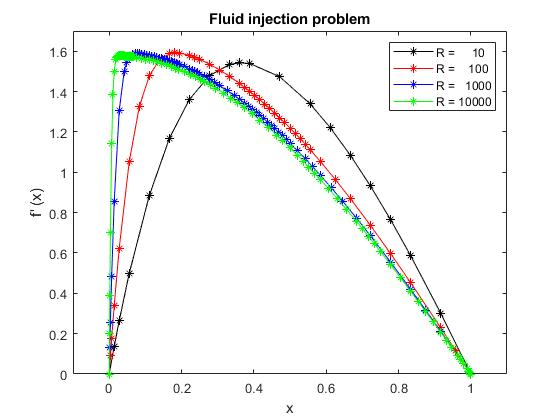
\includegraphics[width=8cm]{fig1.jpg}
\end{center}
\caption{Prikaz rješenja za različite R}
\end{figure}

Promotrimo samo na slici malo mrežu kada se približavamo $x=0$, $*$ su označenje točke, primijetimo koliko su gušće za vrijednosti blizu $x=0$ za različite vrijednosti $R$, to u upravo granični sloj (boundary layer).
Rezultati za nepoznate vrijednosti parametra $A$ za odgovarajuće vrijednosti Reynoldsovog broja su dane u sljedećoj tablici.

\begin{center}
\begin{tabular}{|| c | c ||}
 \hline
  R & A\\
 \hhline{|=|=|}
 10 & 3.81\\
 \hline
 100 & 2.76\\
 \hline
 1000 & 2.55\\
 \hline
 10000 & 2.49\\
 \hline
\end{tabular}
\end{center}

\bibliographystyle{plain}
\bibliography{bibliography.bib}
\end{document}